% !TeX encoding = UTF-8
% !TeX spellcheck = es_ES
% !TeX root = ../ComponentCatalog.tex
%!TEX root=../ComponentCatalog.tex

\begin{table}[H]
    \centering
    \renewcommand\theadfont{\bfseries}
    \setlength{\tabcolsep}{10pt}
    \renewcommand{\arraystretch}{1.5}

    \begin{tabular}{|c|c|c|c|}
        \hline
        \multicolumn{4}{|c|}{\thead[b]{Botones SMD Amazon}} \\
        \hline

        \multicolumn{4}{|c|}{
            \begin{tikzpicture}[baseline=0]
                \draw (0,0) rectangle (10,10);
                \begin{scope}
                    \clip (0,0) rectangle (13,10);
                    \node[inner sep=0pt] at (6,5.5)
                        {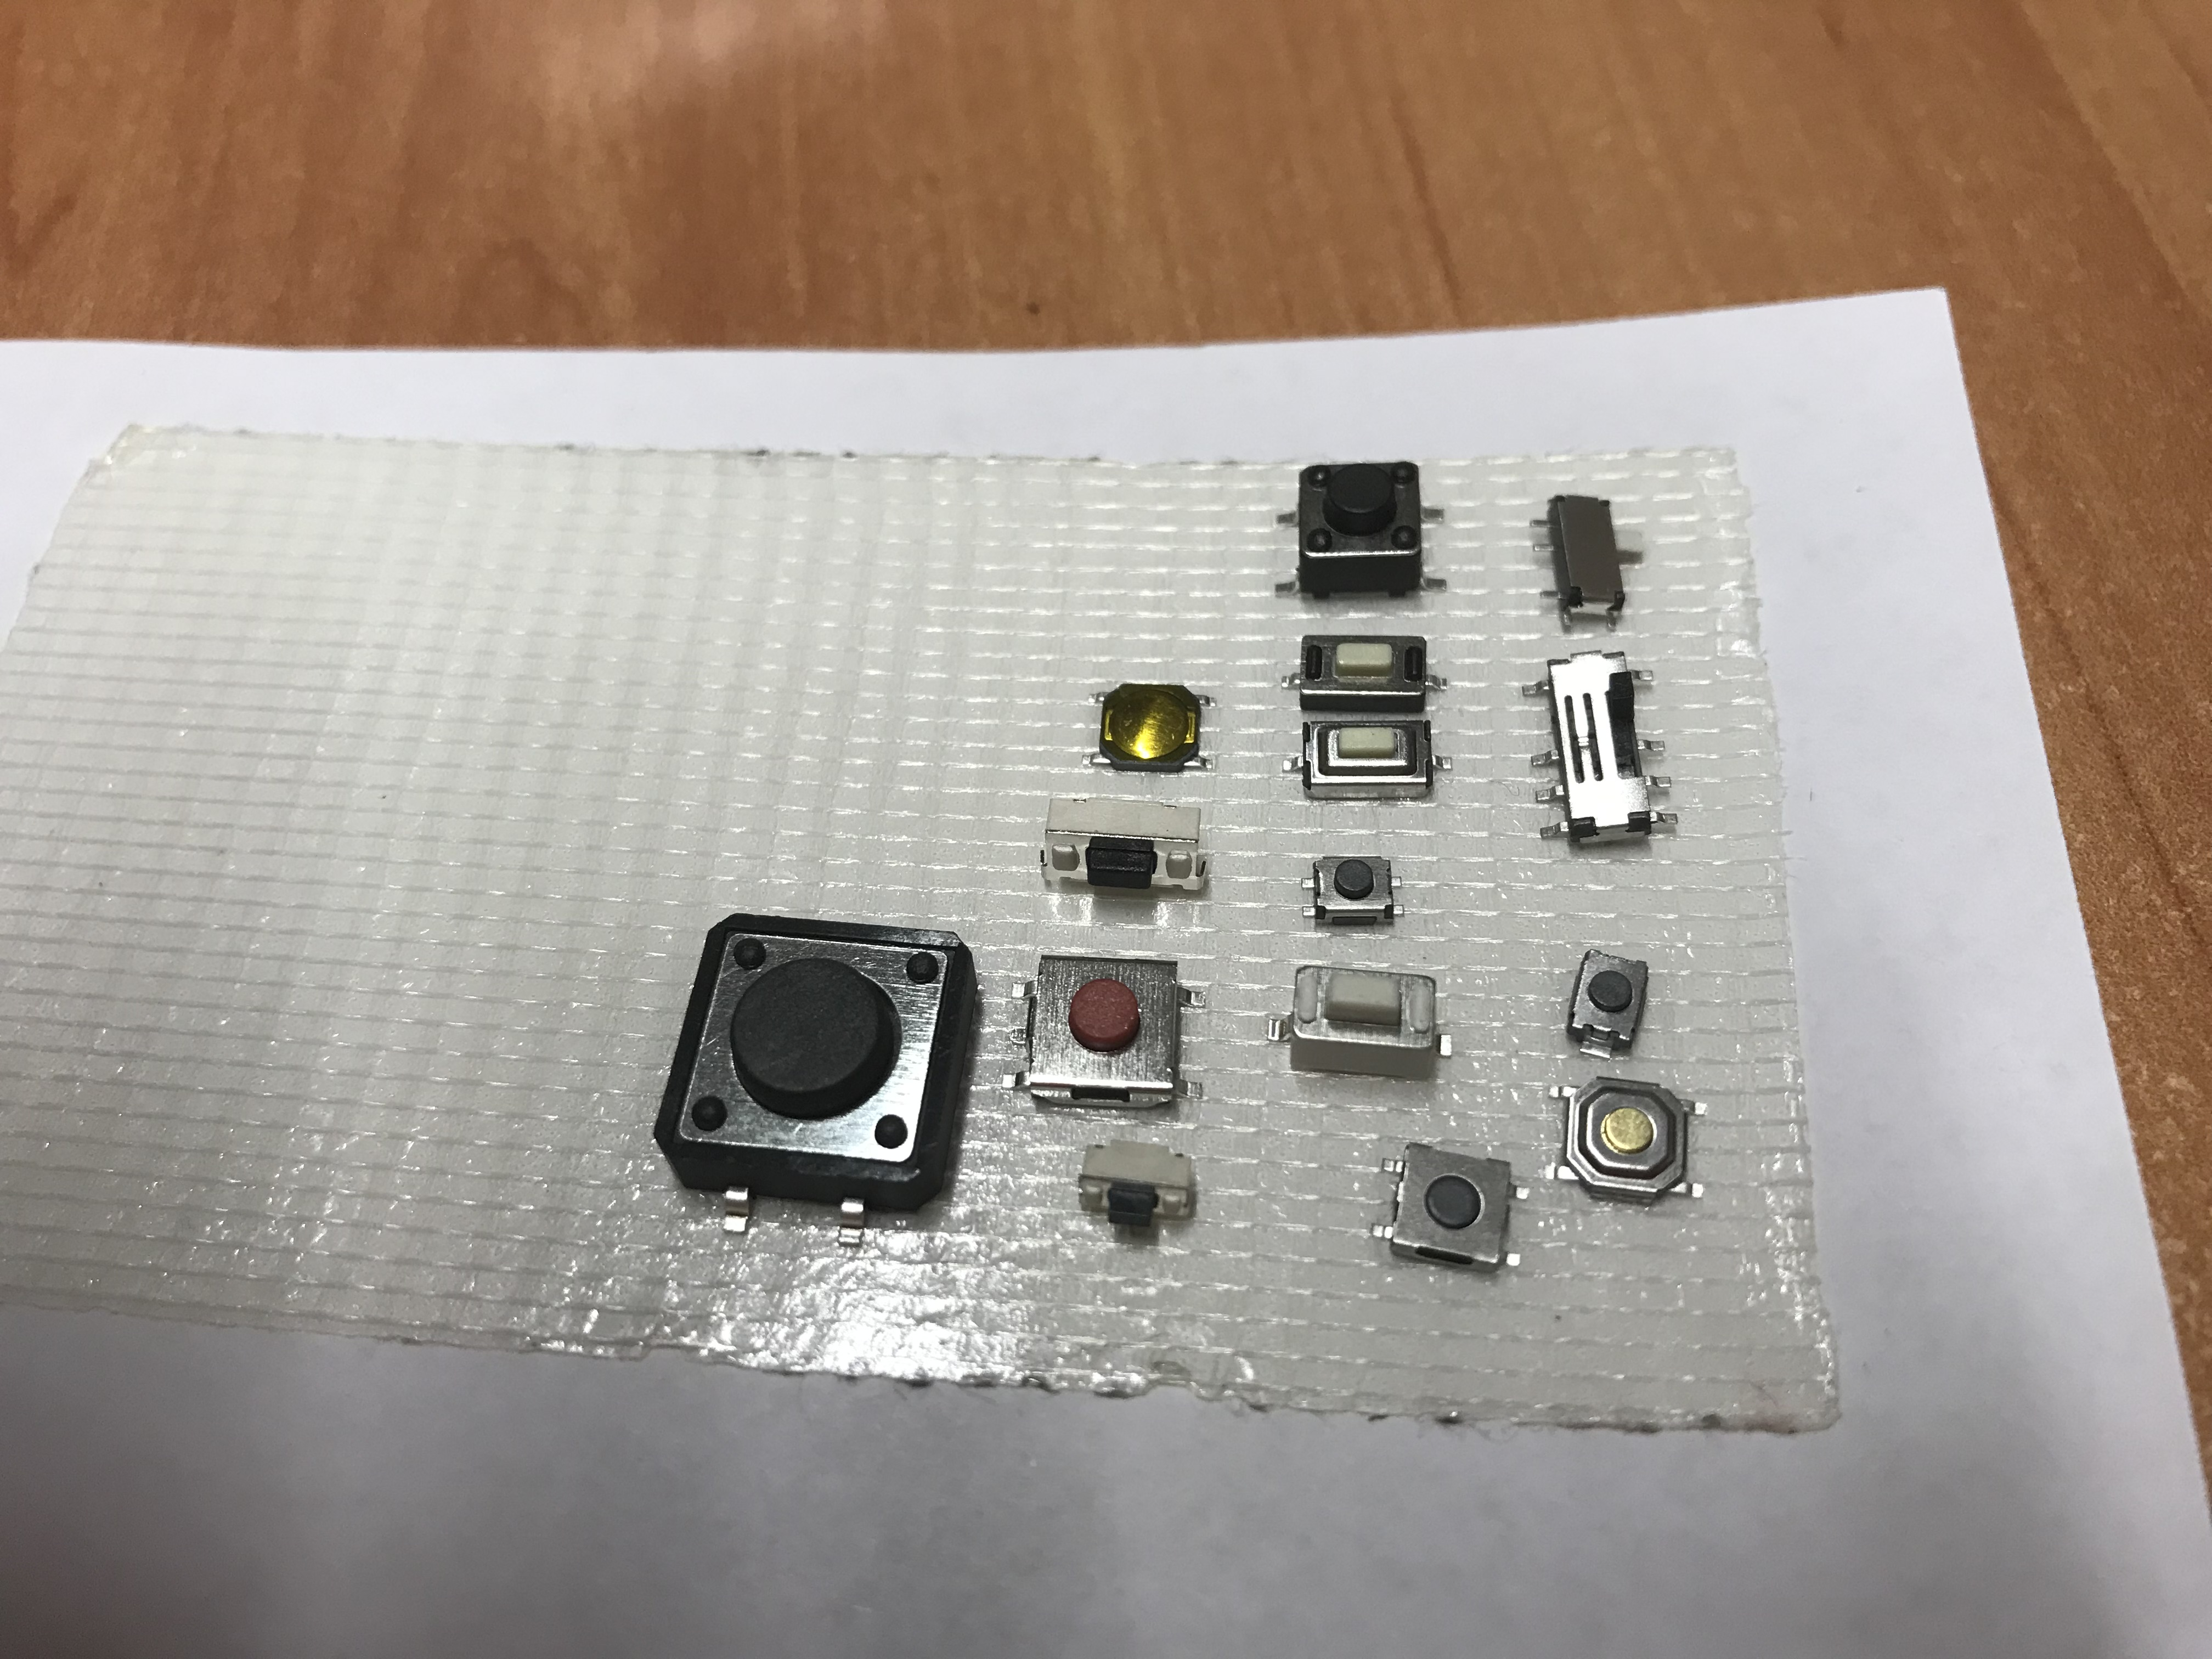
\includegraphics[scale=.175]{pictures/smdBtn.jpg}};
                \end{scope}
                \addvmargin{1mm}
            \end{tikzpicture} 
        } \\
        \hline

        & & 6x6x3.5 &SPST 6.6x2.7x1 \\ \hline
        & & 6x3.5x1.5 (B) &  \multirow{2}{*}{DT3P 8x3.5x1.5}\\ \cline{1 - 3}
        & 4.5x4.5x0.7 (D) & 6x3.5x1.5 (B) & \\ \hline
        & 7x2.5x3.3 [L]& 3.3x2.8x1.2 &  \\ \hline
        \multirow{2}{*}{12x12x3} & 6.5x6.5x2 (R) &6x3.5x3.3(B) &3.8x3x1.3\\ \cline {2 - 4}
        & 4.5x2.3x2 (L)&4.5x4.5x1 & 5x5x1 (D) \\ \hline 
        \thead[b]{Uso} & \multicolumn{3}{|l|}{Tener Catalogo Botones para buscar}\\ \hline
        \thead[b]{Ubicacion} & \multicolumn{3}{|l|}{TR}\\ \hline

    \end{tabular}
    \caption{Botones SMD Amazon}
    \label{tab:BtnSmdAmazon}
\end{table}


